\subsubsection{\texttt{RN-5}: migración a GitHub Actions del sistema de integración continua}
\label{subsec:rn5}

Previamente al inicio del presente Trabajo Fin de Grado, el proyecto \textit{VSCode4Teaching} hacía uso de un sistema de integración y despliegue continuos a través de \textbf{Travis CI} en el que recaían tres tareas: cada vez que se producían modificaciones en la rama \texttt{master}, se ejecutaban las pruebas automáticas de servidor y extensión y, además, se publicaban nuevas etiquetas de la imagen del servidor en el repositorio en Docker Hub.

Este sistema se ha visto reemplazado por GitHub Actions, descrito en la \referenciaSeccion{subsec:herCiCd}. Sin embargo, esta migración no se ha limitado a replicar la funcionalidad previamente utilizada en el sistema de integración, entrega y despliegue continuos sino que, además, se ha aprovechado para ampliar su alcance.

Como consecuencia, el proyecto \textit{software} de \textit{VSCode4Teaching} cuenta ahora con dos flujos de trabajo (\textit{workflows}) diferenciados por componentes. El primero de estos, dedicado a las tareas relativas al servidor y la aplicación web, cuenta con tres trabajos definidos:
\begin{itemize}
    \item \texttt{Test}. Es el trabajo encargado de la ejecución de la batería de pruebas automáticas implementada en el servidor. Se ejecuta cada vez que se produce una alteración en las ramas \texttt{master} o \texttt{develop} del proyecto y, además, cuando se produce un \textit{pull request}\footnote{\textit{Pull request}. En su origen, solicitud realizada al propietario legítimo de un código para realizar una incorporación de otro código implementado fuera del repositorio original. Actualmente, además, se utiliza como sistema organizativo que permite coordinar la fusión de las distintas ramas de un repositorio y dotar a este proceso de un entorno que permite debates entre programadores, solicitar aprobaciones y ejecutar validaciones automáticas, entre otros.} entre ellas para conocer el estado de las pruebas antes de fusionar cambios a la rama del código de producción.
    \item \texttt{Publish}. Se encarga de la publicación de las nuevas versiones lanzadas al repositorio en Docker Hub y, por tanto, se ejecuta cada vez que se modifica la rama \texttt{master}. Genera una imagen Docker utilizando la declaración existente en el proyecto (véase la \referenciaSeccion{subsec:rn4}) y la publica en el repositorio del proyecto en Docker Hub, liberando dos etiquetas: actualiza la versión \textit{latest} de la imagen y, además, genera una nueva específica para la versión liberada.
    \item \texttt{Deploy}. Una vez publicada una nueva versión en Docker Hub, se accede mediante SSH\footnote{SSH. Siglas de ``terminal seguro'' (del inglés \textit{Secure SHell}). Es un protocolo utilizado para la administración remota de computadores.} a la máquina de producción, le transfiere una nueva versión del fichero Docker Compose en la que se utiliza la nueva versión puesta en producción, descarga la imagen desde Docker Hub y aplica los cambios al despliegue, dejando activa en producción la nueva versión automáticamente.
\end{itemize}

Análogamente, se declara un flujo de trabajo para la extensión que comprende únicamente los dos primeros trabajos descritos para el caso anterior, particularizándolos para la plataforma \textit{software} que emplea este componente. De este modo, para la extensión se ejecuta la batería de pruebas automáticas tras cada \textit{commit} en las ramas \texttt{master}, \texttt{develop} y cuando se produzca un \textit{pull request} entre ellas y, si se ha lanzado una nueva versión, se publica automáticamente en el Visual Studio Code Marketplace.

Todos los flujos anteriormente descritos quedan declarados en sendos ficheros YAML dentro del directorio \texttt{.github/workflows} en el proyecto, siendo esta la ubicación requerida por GitHub Actions para ejecutarlos automáticamente. Sirva como ejemplo el \referenciaCodigo{cod:ciGitHubTestServer}, que es la especificación para GitHub Actions del trabajo que ejecuta las pruebas automáticas del servidor, que es el primero de los especificados en el fichero \texttt{server.ci.yml}.

\begin{lstlisting}[language=YAML,caption={Fragmento del flujo de trabajo de acciones automáticas relativas a la integración continua del servidor.},label=cod:ciGitHubTestServer]
name: "Server pipeline"

on:
  push:
    branches:
      - master
      - main
      - develop
  pull_request:
    branches:
      - master
      - main
      - develop

jobs:
  test:
    runs-on: ubuntu-latest
    defaults:
      run:
        working-directory: ./vscode4teaching-server
    steps:
      - name: Checkout repository
        uses: actions/checkout@v4
      - name: Set up Java version
        uses: actions/setup-java@v4
        with:
          java-version: 11
          distribution: temurin
      - name: Test
        run: ./mvnw clean dependency:resolve test
  publish:
    if: ${{ github.event_name == 'push' && github.ref == 'refs/heads/main' }}
    needs: test
    # [...]   
  deploy:
    if: ${{ github.event_name == 'push' && github.ref == 'refs/heads/main' }}
    needs: publish
    # [...]
\end{lstlisting}

En la \referenciaFigura{fig:reqn5-1} se muestra una parte del histórico de ejecuciones de los flujos de trabajo definidos para varios \textit{commits} ejecutados sobre la rama \texttt{develop}. GitHub Actions posibilita acceder al detalle de cada ejecución, permitiendo visualizar gráficamente el estado y disposición de los trabajos realizados. Además, en caso de ser necesario, también se pueden obtener los registros en detalle de la ejecución de cada uno de los trabajos que componen un flujo.

\begin{figure}[h]
    \centering
    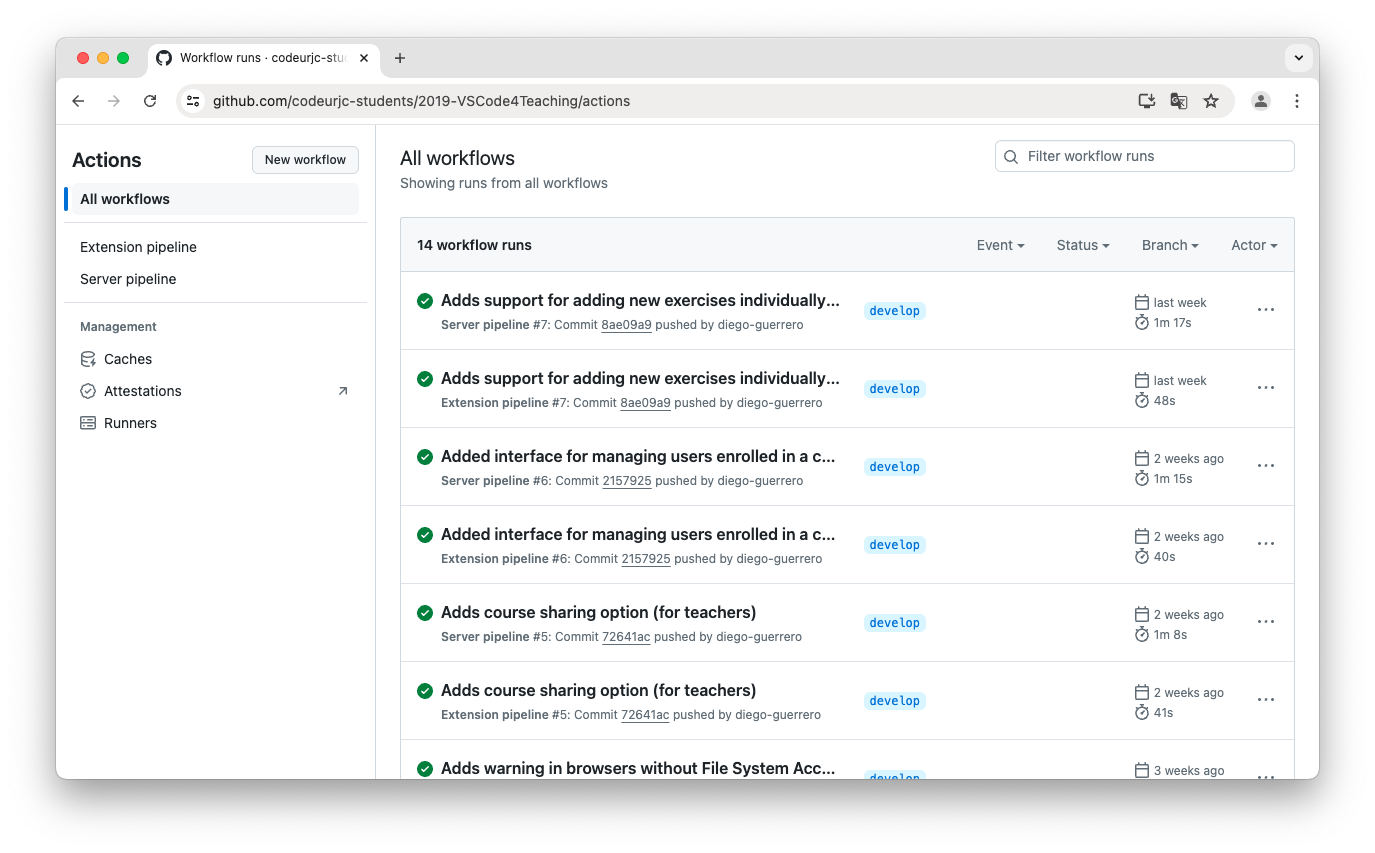
\includegraphics[width=\textwidth]{imagenes/utilizadas/4-3-implementacion/rn5-1.png}
    \caption{Fragmento del listado de ejecuciones de los flujos de trabajo de integración continua con GitHub Actions.}
    \label{fig:reqn5-1}
\end{figure}
